\subsubsection{UV-Sensor}
Der CubeSat besitzt einen UV-Sensor, aus diesem Grund wurde auch in die Testkammer einer eingebaut. Es wurde der UV-Sensor LTR390\autocite{LTR390} verwendet. Dieser verfügt über einen integrierten ADC, somit muss kein Analog-Digital-Wandler dazwischengeschaltet werden und kann direkt über I2C an den \raspi angeschlossen werden.\\
\vspace{5mm}
\begin{table}[H]
    \centering
    \begin{tabular}{ | c | c | } 
  \hline
   VCC & 5 Volt\\ 
  \hline
   GND & Ground\\ 
  \hline
   SDA & GPIO3 \\ 
  \hline
   SCL & GPIO5 \\ 
  \hline
   INT & Interruptausgang \\ 
  \hline
\end{tabular}
    \caption{Pinbelegung UV-Sensor}
\end{table}
\begin{figwindow}[0,r,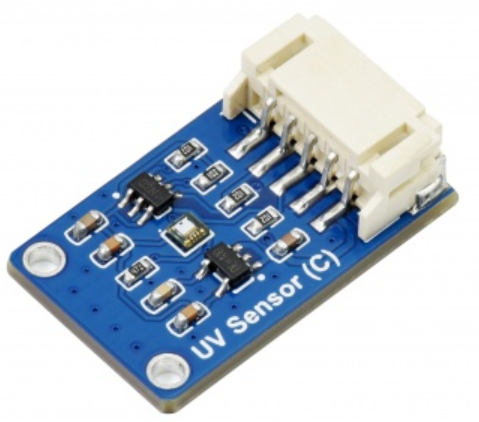
\includegraphics[scale=0.5]{image/UVsensor.png},{UV-Sensor}]
Das Licht der UV-Lampe\ref{sec:UV-Lampe} hat eine Wellenlänge von 385nm bis 400nm. Daher muss der UV-Sensor auch für diesen Bereich ausgelegt sein. Der Messbereich des LTR390 ist zwischen 200nm und 400nm. Der Sensor misst das Umgebungslicht und den UV-Index. Das Umgebungslicht wird in Lux angegeben. Ein niedriger Lux-Wert bedeutet das der Sensor sich in einer dunklen Umgebung befindet. Ein hoher Wert bedeutet eine helle Umgebung. Der UV-Index wird in verschiedene Kategorien eingeteilt.
\end{figwindow}
\vspace{2mm}
\begin{table}[h]
    \centering
    \begin{tabular}{ | c | c | } 
  \hline
   UV-Index & Kategorie\\ 
  \hline
   0-2 & Niedrig\\ 
  \hline
   3-5 & Mäßig \\ 
  \hline
   6-7 & Hoch \\ 
  \hline
   8-10 & sehr Hoch \\ 
  \hline
   11+ & Extrem \\ 
  \hline
\end{tabular}
    \caption{UV-Index}
\end{table}

\begin{figure}[H]
    \centering
    \begin{subfigure}[b]{0.45\textwidth}
        \centering
        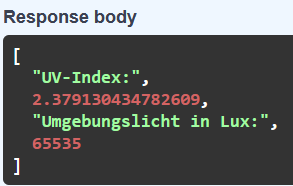
\includegraphics[width=\textwidth]{image/UVsensor hell.png}
        \caption{indirektes Sonnenlicht}
        \label{fig:bild1}
    \end{subfigure}
    \hfill
    \begin{subfigure}[b]{0.45\textwidth}
        \centering
        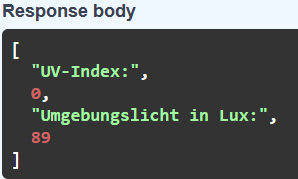
\includegraphics[width=\textwidth]{image/uvsensor dunkel.png}
        \caption{kein Sonnenlicht}
        \label{fig:bild2}
    \end{subfigure}
    \caption{Messungen mit UV-Sensor}
    \label{fig:zwei_bilder}
\end{figure}
Die Messungen der oberen zwei Abbildungen wurden in einem Zimmer durchgeführt. Der Sensor in Abbildung (a) wurde für die Messung dem Sonnenlicht durch ein Fenster ausgesetzt. Aus diesem Grund ist der UV-Index eher niedrig. Der LTR390 kann Umgebungslicht von 0 Lux bis zu 65535 Lux messen. In Abbildung (a) ist zu erkennen, dass der maximale Wert bei der Messung des Umgebungslichtes erreicht wurde. Daraus kann geschlussfolgert werden, dass sich der Sensor in einer hellen Umgebung befunden hat. In Abbildung (b) wurde der Sensor vom Sonnenlicht entfernt, somit haben keine UV-Strahlen den Sensor getroffe. Dies kann auch am gemessenen UV-Index erkennt werden. Es wurde ein Umgebungslicht von 89 Lux gemessen. Der UV-Sensor war also in einer eher dunklen Umgebung.\\
Für den LTR390 UV-Sensor wird die folgende Bibliothek\autocite{LTR390} verwendet:
\begin{verbatim}
pip install adafruit-circuitpython-ltr390
\end{verbatim}
\vspace{3mm}
Das Testprogramm für den UV-Sensor ist im Kapitel \ref{sec:Testprogramm UV-Sensor} und der Codeabschnitt für die API im Kapitel \ref{API-UVS}